\documentclass{article}
\usepackage{amsmath}
\usepackage{graphicx}
\usepackage{geometry}
\geometry{margin=1in}

\title{Simulation-Based Inference (SBI) for Linear Regression}
\author{}
\date{}

\begin{document}

\maketitle

\section*{Objective}
This experiment applies Simulation-Based Inference (SBI), along with analytic and MCMC methods, to solve a simple linear regression problem where the goal is to infer the posterior distribution over the slope and intercept of a line given noisy observations.

\begin{figure}[h]
    \centering
    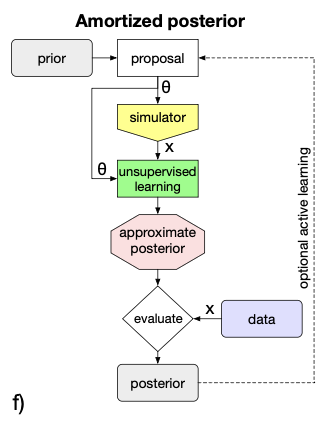
\includegraphics{SBIapproach.png}
    \caption{SBI approach used in the linear regression problem}
\end{figure}
\section*{What is SBI?}
\textbf{Simulation-Based Inference} (SBI) is a class of techniques used to estimate posterior distributions when the likelihood function is intractable or unavailable. Instead of using explicit formulas, SBI trains neural networks on simulations of parameter-data pairs to learn a mapping from observations to posterior distributions.

\subsection*{Bayesian Foundations}
Bayes' Theorem forms the foundation of Bayesian inference:
\[
p(\theta \mid x) = \frac{p(x \mid \theta) \cdot p(\theta)}{p(x)}
\]
where:
\begin{itemize}
    \item $p(\theta)$ is the prior belief about the parameters $\theta$
    \item $p(x \mid \theta)$ is the likelihood of observing data $x$ given parameters $\theta$
    \item $p(\theta \mid x)$ is the posterior distribution of parameters given the observed data
    \item $p(x)$ is the marginal probability of the data
\end{itemize}

\subsection*{The Problem}
In many real-world applications, we can simulate data $x$ from a model given parameters $\theta$, but we cannot write down or compute the likelihood $p(x \mid \theta)$. This makes classical Bayesian inference difficult or impossible.

\subsection*{The SBI Solution}
Simulation-Based Inference (SBI) bypasses the need for an explicit likelihood. The idea is to use simulations to learn the relationship between parameters and data. The process works as follows:

\begin{enumerate}
    \item Sample $\theta$ from the prior distribution
    \item Simulate data $x$ from the model using $\theta$
    \item Train a neural network to learn how $\theta$ and $x$ relate
    \item Once trained, input the observed data $x_{\text{obs}}$ into the network to obtain the posterior $p(\theta \mid x_{\text{obs}})$
\end{enumerate}

\subsection*{(S)NPE: (Sequential) Neural Posterior Estimation}
In this experiment, we use SNPE, which learns the posterior distribution $p(\theta \mid x)$ directly from simulations. This is done using a conditional density estimator (e.g., a neural network) trained on many $(\theta, x)$ pairs.

SBI is especially useful when:
\begin{itemize}
    \item The likelihood function is unknown or too complex to compute.
    \item The model is a simulator. Simulator is a computer program that
    takes as input a vector of parameters $\theta$, samples a series of
    internal states or latent variables $z_i \sim p_i(z_i|\theta,z_{<i})$, and finally
    produces a data vector $x\sim p(x|\theta,z)$ as output. The simulator mimics a real-world process by stochastically generating internal states (latent variables) and then producing observable data — and this process is what SBI methods rely on to learn about $\theta$ from observed x.
    \item You still want to do Bayesian inference and get full posterior distributions.
\end{itemize}

SBI allows Bayesian reasoning even when traditional tools break down.
Specifically, the algorithm used here is Sequential Neural Posterior Estimation (SNPE), which learns a conditional density estimator over parameters given data.
The \textbf{amortized posterior approach} (figure 1), used here, is a simulation-based inference technique where a neural network is trained to approximate the posterior distribution over model parameters given observed data. This is achieved by first drawing parameter samples from a prior and using them to generate synthetic data through a simulator. The resulting (parameter, data) pairs are used to train a neural density estimator, such as in Sequential Neural Posterior Estimation (SNPE), which learns to model the posterior directly. Once trained, this network can quickly produce posterior estimates for new observations without retraining, making the inference process highly efficient and reusable. This "amortization" of inference is especially useful in scenarios where inference needs to be performed repeatedly or in real-time.
\textbf{Supervised learning} is a machine learning approach where the model is trained on input-output pairs, meaning it learns to map inputs to known labels.
The focus is on modeling a distribution, not classifying or regressing to known labels.
There's no "true" label for a real-world x; instead, the simulator is used to generate synthetic data, and the model learns the structure of the posterior from this.
It's framed as density estimation — learning to approximate $p(x \mid \theta)$, which is a typical goal in unsupervised learning.
So while technically we do use paired data during training, the learning goal aligns more with unsupervised learning: discovering a latent distribution rather than predicting a fixed label.
\subsection*{Normalizing Flows}
Normalizing flows are a class of neural density estimation models that transform a simple base distribution (e.g., a multivariate Gaussian) into a complex target distribution using a sequence of invertible and differentiable transformations. Given a base variable $\mathbf{u} \sim p(\mathbf{u})$ and an invertible function $\mathbf{x} = g_\phi(\mathbf{u})$, the probability density of $\mathbf{x}$ under the model, denoted $p_g(\mathbf{x})$, is computed using the change-of-variables formula: $p_g(\mathbf{x}) = p(\mathbf{u}) \left| \det \left( \frac{\partial g_\phi^{-1}(\mathbf{x})}{\partial \mathbf{x}} \right) \right|$. The parameters $\phi$ of the transformation are optimized by maximizing the likelihood of the observed data. Normalizing flows are expressive, scalable to high-dimensional data, and enable both efficient sampling and likelihood evaluation, making them well-suited for simulation-based inference tasks.

\section*{Experimental Setup}
\begin{itemize}
    \item True parameters: slope = 3.6, intercept = -4.4
    \item Noise level: $\sigma = 0.1$
    \item x-values: 30 points evenly spaced in $[-1, 1]$
    \item Prior bounds: Uniform over $[-7, 7]$ for both parameters
    \item Number of simulations: 3000
    \item Posterior samples: 10,000
\end{itemize}

\section*{Findings}
Our code does not operate in the i.i.d, it uses a single observation composed of multiple data points ($y\_obs = sim\_wrapper(theta\_true)$). The likelihood in your case does not factorize over multiple independent samples, but rather is based on the joint likelihood over all elements of that single vector x.
\paragraph{Traditional Methods (for expected questions)} 
Traditional approaches to likelihood-free inference include Approximate Bayesian Computation (ABC) and classical density estimation. ABC approximates the posterior by drawing parameters from the prior, simulating data, and accepting parameter samples if the simulated data is sufficiently close to the observed data, based on a distance metric and a tolerance threshold. While simple, ABC becomes inefficient in high dimensions and lacks amortization, requiring the full procedure to be rerun for each new observation. In contrast, density estimation methods approximate the likelihood function by modeling the distribution of simulated data using techniques like histograms or kernel density estimation. This allows for amortized inference—after the initial computational cost of simulation and density estimation, new data can be processed efficiently. However, both methods depend heavily on hand-crafted, low-dimensional summary statistics and struggle with high-dimensional data due to the curse of dimensionality.

\subsection*{1. Posterior Consistency}
The posterior distributions estimated by SBI, the analytic solution, and MCMC agree very closely. The scatter plot in parameter space shows that all three methods recover a similar elliptical region of high probability mass centered around the true parameters.

\subsection*{2. Posterior Predictive Check}
Regression lines sampled from the SBI posterior densely overlap the true regression line. The variation in these lines reflects the uncertainty in the inferred parameters, and the true line lies well within this range.

\subsection*{3. Pairplots}
The pairplots of SBI, analytic, and MCMC samples all exhibit tight, elliptical shapes indicating low uncertainty. There's a noticeable negative correlation between slope and intercept, typical in linear regression with Gaussian noise.

\subsection*{4. Training Behavior}
The SBI validation loss curve demonstrates steady convergence with some noise, which is expected due to the stochastic nature of training. The posterior learned by SBI is sharp and precise, suggesting that 3000 simulations were sufficient for this problem.

\section*{Conclusions}
SBI performs excellently in this controlled linear regression setting, achieving posterior estimates nearly identical to those from analytic Bayesian inference and MCMC.

The use of narrowed prior bounds and sufficient simulations ensures that the neural density estimator converges reliably, even without explicit seed-setting. SBI is a powerful and flexible approach when the likelihood is unknown, and this experiment validates its performance in a simple, interpretable setting.

\section*{Suggestions}
\begin{itemize}
    \item For more complex models or higher-dimensional problems, consider increasing the number of simulations and using more expressive density estimators like Neural Spline Flows (NSF).
    \item Although the results are stable here, enforcing reproducibility via fixed seeds or deterministic simulation setups may be recommended in critical applications.
\end{itemize}

\section{Presentation Structure}
The following contents will be added in the Presentation:
\begin{enumerate}
    \item Contents (0.5min)
    \item Introduction to the SBI problem (2min)
    \item Linear Regression Problem - Analysis of the findings and plots (2min)
    \item Correlation and Intro to the Gravitational Waves Inference problem (1min)
    \item GW code Analysis of the findings and plots (3min)
    \item Conclusions (1min)
\end{enumerate}

\end{document}
